% !TEX root = main.tex
\begin{figure*}[t]
    \centering
    \begin{subfigure}[t]{0.3\textwidth}
        \centering
        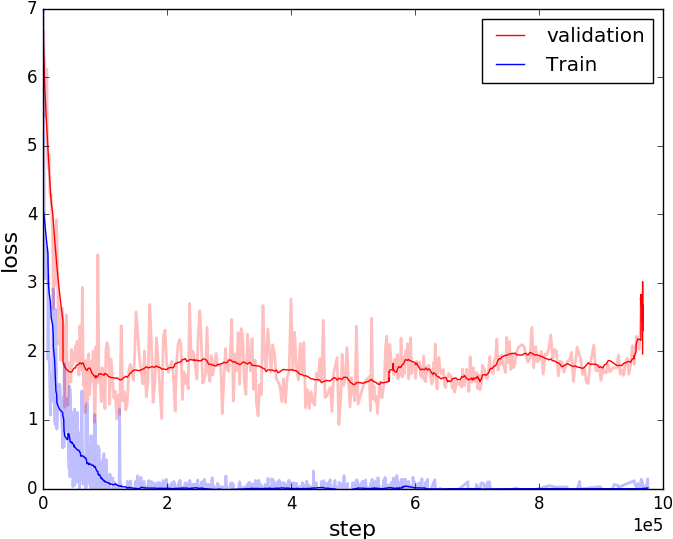
\includegraphics[height=3.5cm]{Images/step_m1f1.png}
        \caption{\label{fig:m1f1}\mone-\fone}
    \end{subfigure}%
    ~
    \begin{subfigure}[t]{0.3\textwidth}
        \centering
        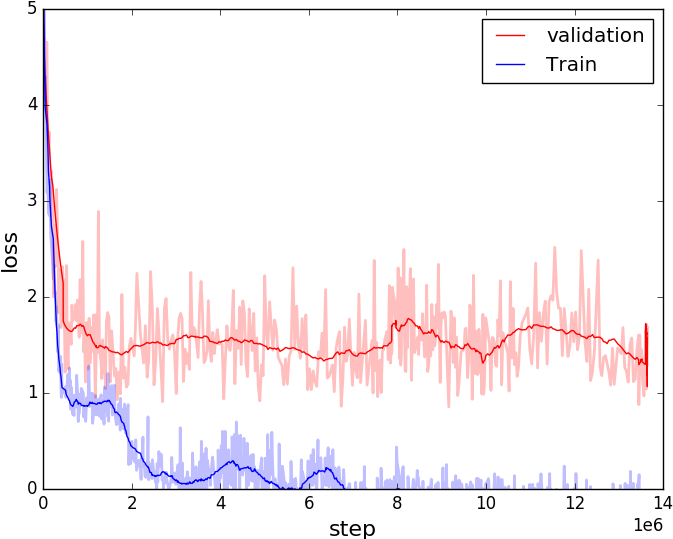
\includegraphics[height=3.5cm]{Images/step_m1f2.png}
        \caption{\label{fig:m1f2}\mone-\ftwo}
    \end{subfigure}%
    ~
    \begin{subfigure}[t]{0.3\textwidth}
        \centering
        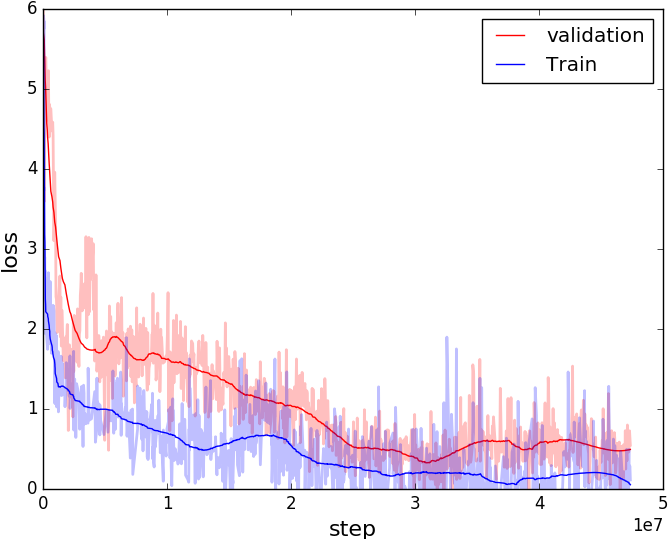
\includegraphics[height=3.5cm]{Images/step_m1f3.png}
        \caption{\label{fig:m1f3}\mone-\fthree}
    \end{subfigure}%
    \\
    \begin{subfigure}[t]{0.3\textwidth}
        \centering
        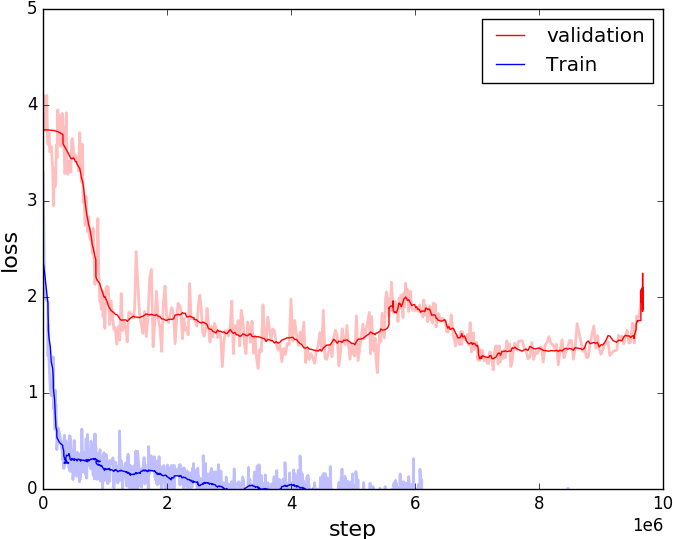
\includegraphics[height=3.5cm]{Images/step_m2f1.png}
        \caption{\label{fig:m2f1}\mtwo-\fone}
    \end{subfigure}%
    ~
    \begin{subfigure}[t]{0.3\textwidth}
        \centering
        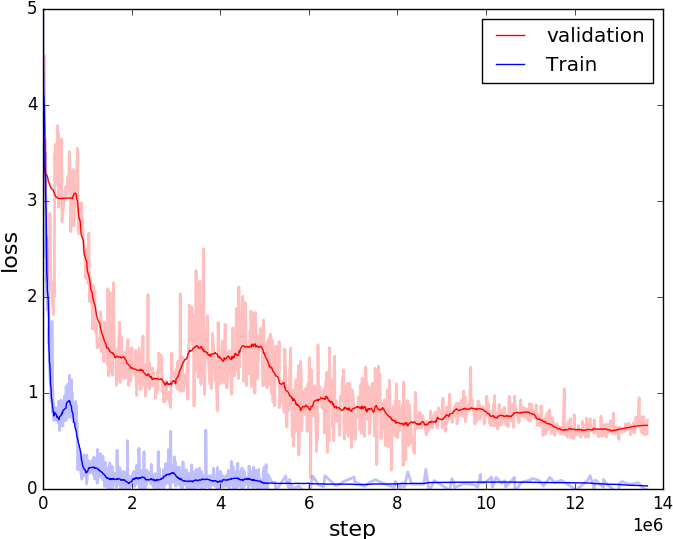
\includegraphics[height=3.5cm]{Images/step_m2f2.png}
        \caption{\label{fig:m2f2}\mtwo-\ftwo}
    \end{subfigure}%
    ~
    \begin{subfigure}[t]{0.3\textwidth}
        \centering
        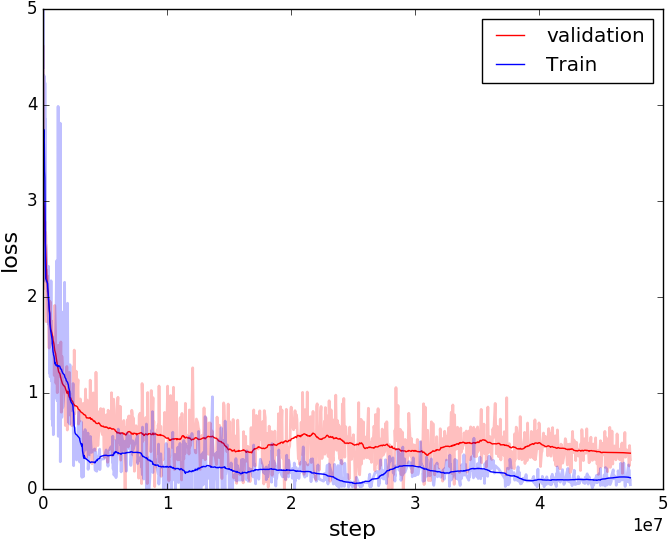
\includegraphics[height=3.5cm]{Images/step_m2f3.png}
        \caption{\label{fig:m2f3}\mtwo-\fthree}
    \end{subfigure}%
        \\
    \begin{subfigure}[t]{0.3\textwidth}
        \centering
        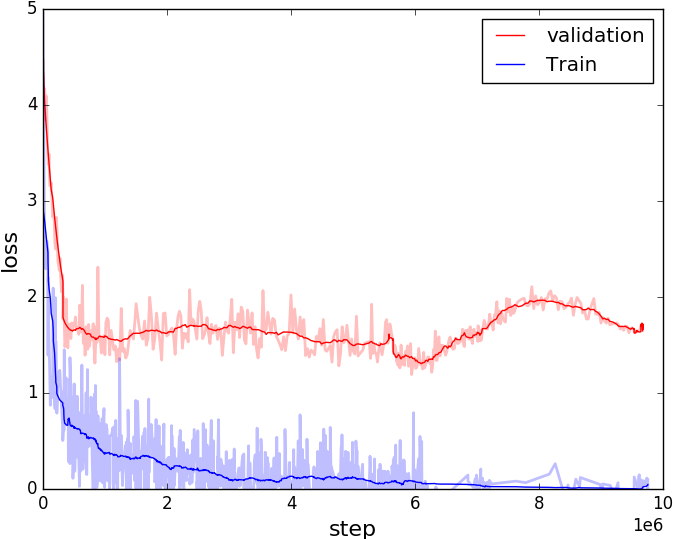
\includegraphics[height=3.5cm]{Images/step_m3f1.png}
        \caption{\label{fig:m3f1}\mthree-\fone}
    \end{subfigure}%
    ~
    \begin{subfigure}[t]{0.3\textwidth}
        \centering
        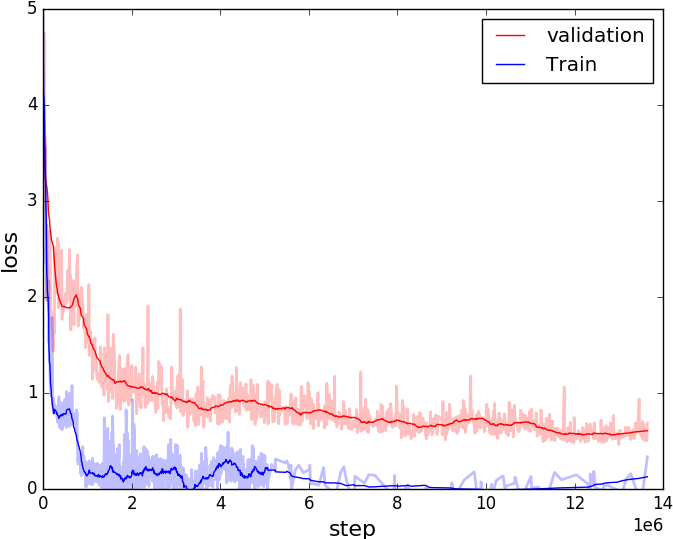
\includegraphics[height=3.5cm]{Images/step_m3f2.png}
        \caption{\label{fig:m3f2}\mthree-\ftwo}
    \end{subfigure}%
    ~
    \begin{subfigure}[t]{0.3\textwidth}
        \centering
        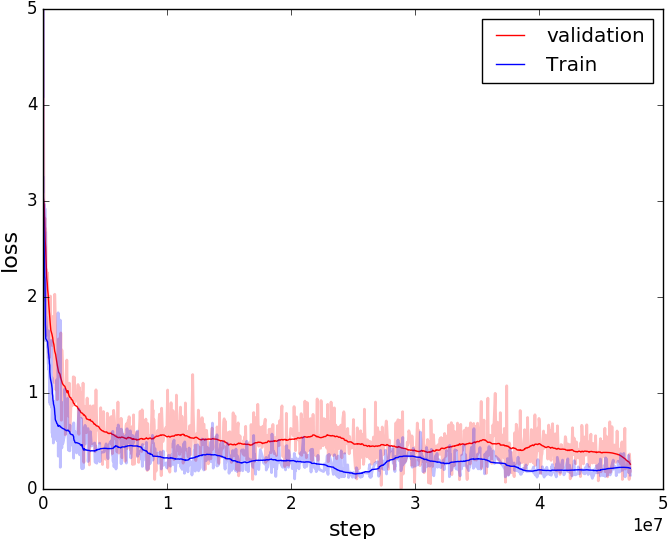
\includegraphics[height=3.5cm]{Images/step_m3f3.png}
        \caption{\label{fig:m3f3}\mthree-\fthree}
    \end{subfigure}%
    \vspace{-5pt}
    \caption{Training and validation loss curves for all combinations of different ranking architectures and feeding paradigms.}
    \label{fig:step-loss}
    \vspace{-5pt}
\end{figure*}
